\documentclass[10pt]{article}
\usepackage[utf8]{inputenc}
\usepackage{hyperref}
\usepackage[pdftex]{graphicx}
    
\title{\textbf{Report on Big Data project: \\Movie Ratings and Tags Analysis}}

\author{
	Bombardi Tommaso - Mat. 904212\\
	Mascellaro Maria Maddalena - Mat. 904213}
\date{\today}

\begin{document}
\maketitle
\newpage
\tableofcontents
\newpage

\section{Introduction}

\subsection{Dataset description}

MovieLens\footnote{\url{https://movielens.org/}} è un servizio di recommendation che consiglia film ai propri utenti, in base alle loro preferenze, e che utilizza dei filtri basati sulle valutazioni e sulle recensioni lasciate dagli utenti. I ricercatori di GroupLens hanno raccolto e reso disponibili i dataset raccolti da MovieLens\footnote{\url{https://grouplens.org/datasets/movielens/}}. Uno di questi, \textit{recommended for education and development}, descrive l'attività di classificazione a 5 stelle e di tagging a testo libero di MovieLens ed è stato usato per questo elaborato.

Il dataset contiene circa 58 mila film, relativamente ai quali sono disponibili 27 milioni di valutazioni e un milione di applicazioni di tag, rilasciate all'incirca da 280 mila utenti. Questi dati sono stati creati dagli utenti di MovieLens in un periodo compreso tra 1995 e 2018 e sono contenuti in più file \textit{csv}, presenti nello zip \textit{ml-latest.zip} (\url{https://grouplens.org/datasets/movielens/latest/}).

Per le interrogazioni realizzate in questo elaborato, sono state considerate tre tabelle presenti all'interno del dataset (volume totale pari a 764 MB):

\begin{itemize}
\item \textit{Movies}, contenente le informazioni relative ai film.
\item \textit{Ratings}, in cui sono presenti le valutazioni assegnate dagli utenti.
\item \textit{Tags}, che comprende le applicazioni di tag testuali ai film.
\end{itemize}

\begin{figure}[th]
	\centering
	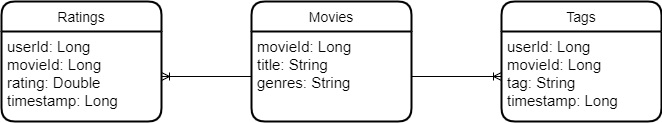
\includegraphics[scale=0.90]{images/MovieLensER.jpg}
	\caption{Diagramma ER relativo alle tabelle del dataset considerate}
\end{figure}

\subsubsection{File description}

Le tre tabelle descritte nella sezione precedente sono contenute nei seguenti file:

\begin{itemize}
\item \textit{movies.csv}, in cui per ogni film è memorizzato un identificativo \textbf{movieId}, una stringa \textbf{title} che rappresenta il titolo e una stringa \textbf{genres} contenente la lista dei generi associati al film separati dal carattere ``\textbar''.
\item \textit{ratings.csv}, in cui per ogni valutazione è presente un record contenente un identificativo \textbf{userId} relativo all'utente responsabile della recensione (nel dataset non sono disponibili altre informazioni sugli utenti), un \textbf{movieId} relativo al film oggetto della valutazione, un punteggio \textbf{rating} con possibili valori compresi tra 0.5 e 5 e un \textbf{timestamp} con le informazioni temporali.
\item \textit{tags.csv}, in cui per ogni applicazione di un tag viene registrato uno \textbf{userId} contenente l'identificativo dell'autore del tag, un \textbf{movieId} che rappresenta il film a cui è associato il tag, un campo di testo \textbf{tag} contenente il tag vero e proprio e un \textbf{timestamp} con le informazioni temporali.
\end{itemize}

\section{Data preparation}

I file descritti sono stati caricati su HDFS e sono reperibili nei seguenti percorsi:

\begin{itemize}
\item \textit{Movies}: \texttt{hdfs:/user/mmascellaro/project/movies.csv}.
\item \textit{Ratings}: \texttt{hdfs:/user/mmascellaro/project/ratings.csv}.
\item \textit{Tags}: \texttt{hdfs:/user/mmascellaro/project/tags.csv}.
\end{itemize}

I dati non sono di scarsa qualità e non contengono una quantità significativa di informazioni inutili, perciò non è stata eseguita una fase di pre-processing volta a modificare i file \textit{csv} prima di eseguire i job in MapReduce e in Spark. La loro implementazione è in grado di processare direttamente il dataset.

\section{Jobs}

Le due query previste per l'elaborato sono state realizzate sia usando MapReduce, sia con Spark, sia con SparkSQL. In tutti i casi le interrogazioni sono eseguite in sequenza, così che la seconda (ove possibile e in accordo con quanto previsto dal framework) possa sfruttare i risultati parziali ottenuti dalla prima.

\subsection{Job \#1: Ranking of genres based on the number of movies with an average rating greater or equal to a given thresold}

Il primo job ha l'obiettivo di stilare la classifica dei generi presenti nel dataset, ordinati in base al numero di film appartenenti a quel genere e che hanno ricevuto una valutazione media superiore ad una soglia data (parametro della query).

\subsubsection{MapReduce implementation}

L'implementazione MapReduce usa come input le tabelle \textit{Movies} e \textit{Ratings} e posiziona l'output in \texttt{hdfs:/user/mmascellaro/outputMapReduce/query1/outputX}, dove X è il numero dello stage MapReduce che ha prodotto il risultato.

L'implementazione prevede l'esecuzione sequenziale di 4 job MapReduce, ognuno dei quali utilizza come input o i file che costituiscono il dataset oppure i \textit{SequenceFile} prodotti dal job precedente. L'ultimo job, invece che restituire \textit{SequenceFile}, memorizza l'output prodotto all'interno di un file di testo.

Di seguito, è riportato un diagramma che descrive, ad alto livello, la sequenza e il funzionamento dei 4 job MapReduce implementati (\ref{MapReduce1}).

\begin{figure}[th]
	\centering
	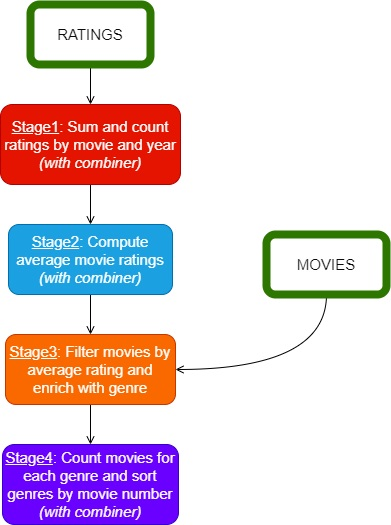
\includegraphics[scale=0.85]{images/MapReduceFlow1.jpg}
	\caption{Stage MapReduce che costituiscono il primo job}
	\label{MapReduce1}
\end{figure}

\begin{itemize}
\item \textbf{Stage \#1} \textit{Sum and count ratings by movie and year}

Questo job prende come input la tabella \textit{Ratings} e restituisce una vista aggregata in cui la chiave è costituita da movieId e anno e il valore da una coppia formata dalla somma delle valutazioni e dal loro numero. A livello implementativo sono stati utilizzati dei combiner, che pre-aggregano i dati dopo l'esecuzione dei task di map e il cui comportamento corrisponde a quello dei reducer (sommano la somma delle valutazioni e il loro numero, possibile perché l'addizione è commutativa e associativa).

Per la risoluzione della prima query questo stage sarebbe eccessivo, perché la valutazione media di ogni film potrebbe essere calcolata direttamente dal file di input. Tuttavia, si è scelto di inserirlo per avere un vantaggio nell'esecuzione della seconda query. Essa, infatti, non dovrà leggere dalla tabella \textit{Ratings} (il file di dimensione maggiore tra quelli usati), ma potrà utilizzare direttamente la vista aggregata ottenuta in questo stage.

Il numero di mapper è uguale a 6 (blocchi HDFS in cui è contenuto il file \textit{Ratings}) ed è stato usato un numero di reducer (valore che può essere passato come parametro al momento dell'esecuzione del job) pari a 4. Il tempo di esecuzione è 1 minuto e 58 secondi (\url{http://isi-vclust0.csr.unibo.it:19888/jobhistory/job/job_1583679666662_4557}).

\item \textbf{Stage \#2} \textit{Compute average movie ratings}

Questo secondo job accetta in input la vista ottenuta con lo stage \#1 ed aggrega ulteriormente i dati eliminando la granularità dell'anno (sia nel passo di map che in quello di reduce la chiave dell'output è il movieId). Il job usa i combiner per eseguire una pre-aggregazione dei dati e infine, nella fase di reduce, calcola la media delle valutazioni assegnate a ciascun film. Nell'output, ad ogni movieId è associata la sua valutazione media.

Il numero di mapper è 4 (reducer dello stage \#1) e, avendo a che fare con una quantità inferiore di dati rispetto allo stage precedente, sono stati usati 2 reducer. Il tempo di esecuzione è 29 secondi (\url{http://isi-vclust0.csr.unibo.it:19888/jobhistory/job/job_1583679666662_4558}).

\item \textbf{Stage \#3} \textit{Filter movies by average rating and enrich with genre}

Il terzo job prende in input il risultato dello stage \#2 ed esegue un filtro sui film, selezionando quelli con una valutazione media superiore alla soglia scelta come parametro della query. Successivamente è prevista un'operazione di join con la tabella \textit{Movies}, utilizzando movieId come chiave del join. Questo stage prevede che nell'output siano presenti tutti i movieId relativi a film con una valutazione media sufficientemente alta, associati alle varie stringhe contenenti i generi assegnati ai film.

Il job utilizza 3 mapper (2 per il risultato dello stage precedente e 1 per la lettura del file \textit{Movies} che, avendo una dimensione ridotta, è contenuto in un solo blocco HDFS) e il numero di reducer scelto è uguale a 2. Il tempo di esecuzione è 26 secondi (\url{http://isi-vclust0.csr.unibo.it:19888/jobhistory/job/job_1583679666662_4559}).

\item \textbf{Stage \#4} \textit{Count movies for each genre and sort genres by movie number}

Questo job accetta in input il risultato dello stage \#3 e, per ogni film dato, il passo di map divide nei vari generi la stringa trovata in precedenza. Il genere diventa la chiave e ad esso viene associato un valore corrispondente al numero di film associati (con valutazione media sufficientemente alta).

L'uso dei combiner scarica parte del lavoro sui task di map, semplificando il compito del reducer. Inoltre, con un solo reducer è possibile ordinare per valore tutti i generi trovati sfruttando il metodo \textit{cleanup}. Esso viene richiamato dal reducer prima di terminare e consente di ordinare i risultati precedentemente calcolati. In MapReduce è previsto un ordinamento per chiave, e \textit{cleanup} consente di modificare l'output prima di emetterlo. Una possibile alternativa sarebbe l'aggiunta di un ulteriore step MapReduce, che inverta chiave e valore sia in fase di map che in fase di reduce.

Il numero di mapper è 2 (reducer dello stage \#3) ed è previsto un solo reducer. A differenza degli stage precedenti in questo job il numero di reducer non può essere settato ad un valore diverso, poiché un solo reducer consente l'ordinamento globale del risultato e la sua memorizzazione in un unico file. Il tempo di esecuzione è 18 secondi (\url{http://isi-vclust0.csr.unibo.it:19888/jobhistory/job/job_1583679666662_4560}).
\end{itemize}

Nella figura che segue (\ref{Result1}) è mostrato un estratto dell'output ottenuto, disponibile nella cartella \texttt{hdfs:/user/mmascellaro/outputMapReduce/query1/output4}.

\begin{figure}[th]
	\centering
	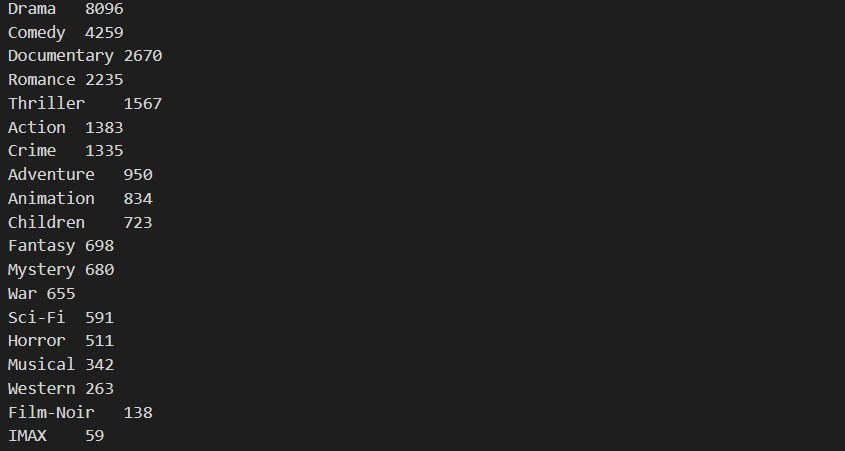
\includegraphics[scale=0.60]{images/Result1.jpg}
	\caption{Output ottenuto con il primo job MapReduce}
	\label{Result1}
\end{figure}

\subsubsection{Spark implementation}

Se paragonata a quella realizzata in MapReduce, l'implementazione in Spark appare molto semplice perché il framework consente di manipolare i dati in modo più diretto e ``naturale''. Le operazioni svolte seguono quanto fatto in MapReduce e, anche in questo caso, per ogni coppia formata da movieId e anno si calcola la vista pre-aggregata contenente la somma delle valutazioni e il loro numero. Essa è poi salvata in memoria tramite un'operazione di \textit{cache}, in modo che anche la seconda query possa lavorare direttamente su questa vista.

Date le dimensioni ridotte della tabella \textit{Movies} (meno di 3 mb), si è scelto di utilizzare una variabile broadcast per memorizzare tutti i record contenuti al suo interno. In particolare, la variabile broadcast è una mappa in cui ad ogni movieId (chiave) è associata una tupla formata dal titolo del film e dalla stringa contenente i generi (valore) ed è stata usata anche nella seconda query.

Il job è stato lanciato con 2 executor (massimo numero consentito dal cluster), 3 core per ogni executor (ogni macchina ha a disposizione 4 core ed uno è stato lasciato libero per l'esecuzione dei demoni) e 2 gb di memoria RAM (1 gb per ogni executor). Se il numero delle partizioni dei file dati in input è maggiore di 12, esso viene posto a 12 (2 per ogni core usato) con un'operazione di \textit{coalesce}, per ottenere una distribuzione migliore dei dati tra le risorse.

Pur avendo lanciato contestualmente la prima e la seconda query, il tempo di esecuzione totale è di 1 minuto e 54 secondi ed è inferiore a quello del solo stage \#1 presente in MapReduce (\url{http://isi-vclust0.csr.unibo.it:18089/history/application_1583679666662_4566/jobs/}). Il risultato ottenuto con Spark è uguale a quello prodotto dal job MapReduce ed è disponibile nella cartella \texttt{hdfs:/user/mmascellaro/outputSpark/query1}.

\begin{figure}[th]
	\centering
	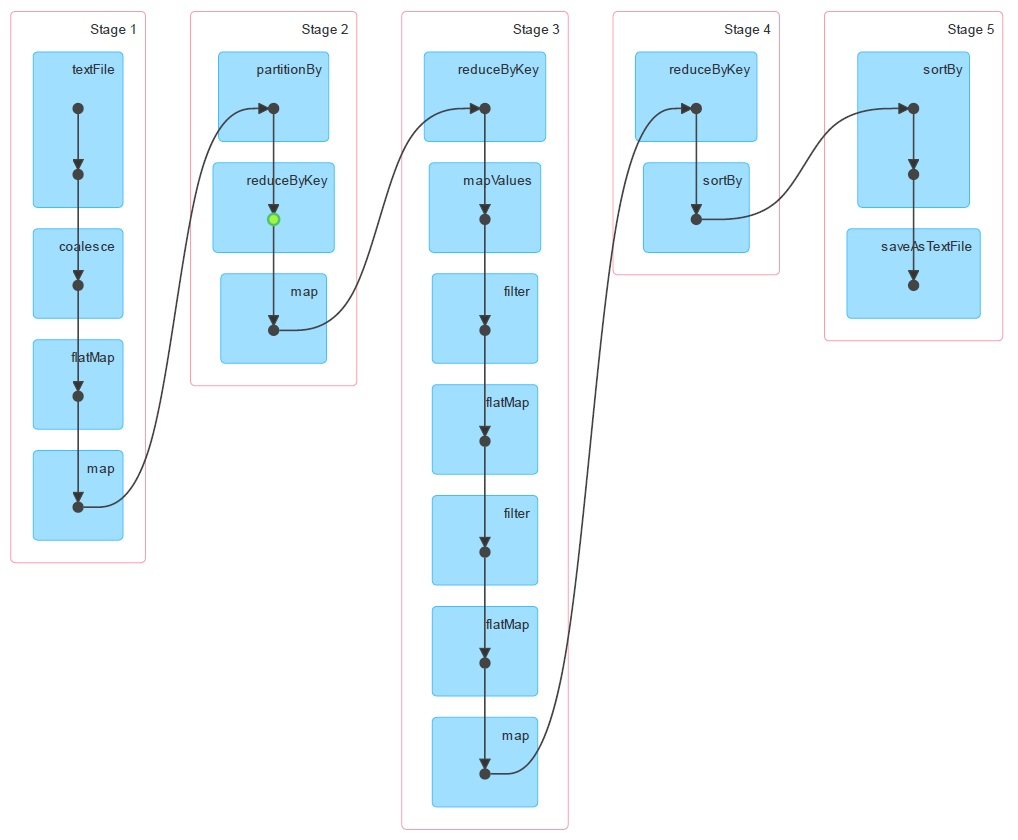
\includegraphics[scale=0.54]{images/DagSpark1.jpg}
	\caption{DAG relativo al primo job Spark}
\end{figure}

\subsubsection{Spark SQL implementation}

In aggiunta alla classica implementazione realizzata con Spark, il job è stato realizzato sfruttando Spark SQL. Questo framework consente di scrivere codice in modo agevole, specialmente se si ha una buona conoscenza di SQL. Questa implementazione è simile alla precedente, con la differenza che vengono costruiti dei \textit{DataFrame} che la query ha il compito di modificare. Come in Spark viene creata e memorizzata tramite \textit{cache} la vista pre-aggregata, mentre per la tabella \textit{Movies} non viene usata una variabile broadcast ma un semplice \textit{DataFrame} (anch'esso salvato in memoria e reso così disponibile alla seconda query).

La configurazione scelta per il job Spark SQL è la stessa usata per Spark (2 executor, 3 core per ogni executor e 2 gb di RAM) e, anche in questo caso, se uno o più file di input sono divisi in più di 12 partizioni viene eseguita l'operazione di \textit{coalesce}. Inoltre, dato che Spark SQL di default usa 200 partizioni nella fase di shuffling, si è scelto di cambiare questo parametro e settarlo a 12.

Il tempo di esecuzione delle due query è di 2 minuti e 6 secondi (\url{http://isi-vclust0.csr.unibo.it:18089/history/application_1583679666662_4567/jobs/}), superiore a quello ottenuto con Spark ma comunque valido dato che in SparkSQL l'ottimizzazione è più complessa. L'output corrisponde a quelli precedenti ed è disponibile nella cartella \texttt{hdfs:/user/mmascellaro/outputSparkSQL/query1}.

\subsection{Job \#2: Top N movies which received the greater number of ratings and tags during each year considered in the dataset}

Il secondo job nasce con l'obiettivo di restituire, per ogni anno considerato nel dataset (1995-2018), i titoli degli N film che hanno ricevuto un numero maggiore di valutazioni e tag da parte degli utenti nel corso di quell'anno. Il valore di N, ossia il numero di film richiesti per ogni anno, è un parametro della query.

\subsubsection{MapReduce implementation}

Nell'implementazione MapReduce l'input è costituito dalle tabelle \textit{Movies}, \textit{Tags} e \textit{Ratings} (quest'ultima non usata direttamente, poiché viene sfruttata la vista pre-aggregata creata nel job precedente) e l'output viene posizionato nella cartella \texttt{hdfs:/user/mmascellaro/outputMapReduce/query2/outputX}, dove X rappresenta il numero dello stage MapReduce che ha prodotto il risultato.

L'implementazione prevede l'esecuzione sequenziale di 4 job MapReduce che sono numerati a partire da 5, poiché sono stati pensati per essere eseguiti in seguito a quelli previsti per il primo job.  È importante sottolineare che la loro esecuzione è possibile soltanto in seguito allo stage \#1 del job precedente (quello che ha il compito di calcolare la vista pre-aggregata contenente le valutazioni).

\begin{figure}[th]
	\centering
	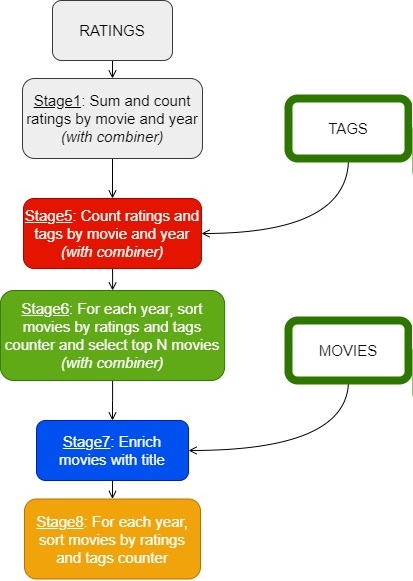
\includegraphics[scale=0.76]{images/MapReduceFlow2.jpg}
	\caption{Diagramma che descrive gli stage MapReduce del secondo job}
\end{figure}

\begin{itemize}
\item \textbf{Stage \#5} \textit{Count ratings and tags by movie and year}

Questo job accetta in input la vista ottenuta con lo stage \#1 mantenendo, per ogni coppia formata da movieId e anno, il numero delle valutazioni ricevute. Inoltre, viene processata la tabella \textit{Tags} in modo che siano contati anche i tag testuali applicati ad un certo film nel corso di un determinato anno. I record ottenuti da entrambi gli input sono uniti (banalmente, si usano due mapper differenti per un solo task MapReduce) e, con l'aiuto dei combiner, viene calcolato il numero totale di feeling (ossia valutazioni e applicazioni di tag) per ogni chiave (movieId e anno).

Il job usa 5 mapper (4 per il risultato dello stage \#1 e 1 per il file \textit{Tags}, che risiede in un unico blocco HDFS) e il numero di reducer scelto è uguale a 2. Il tempo di esecuzione è pari a 32 secondi (\url{http://isi-vclust0.csr.unibo.it:19888/jobhistory/job/job_1583679666662_4561}).

\item \textbf{Stage \#6} \textit{For each year, sort movies by ratings and tags counter and select top N movies}

Il secondo job prende in input il risultato dello stage precedente e, nella fase di map, modifica i record utilizzando l'anno come chiave e la coppia formata da movieId e numero di feeling come valore. Successivamente, per ogni anno vengono ordinati i valori per numero di feeling e selezionati i primi N (N è il parametro della query). Per alleggerire il carico di lavoro dei reducer, sono stati usati dei combiner che restituiscono soltanto N record per ogni task di map. Così i reducer dovranno gestire al più N * M record (e non tutti), dove M corrisponde al numero di mapper.

Il numero di mapper è 2 (reducer dello stage \#5) e sono stati utilizzati 2 reducer, per un tempo di esecuzione di 33 secondi (\url{http://isi-vclust0.csr.unibo.it:19888/jobhistory/job/job_1583679666662_4562}).

\item \textbf{Stage \#7} \textit{Enrich movies with title}

Questo job accetta come input il risultato dello stage \#6 e la tabella \textit{Movies} ed esegue un'operazione di join usando movieId come chiave. Nell'output sono presenti una serie di record aventi come chiave l'anno e come valore la coppia formata da titolo e numero di feeling ma, essendo stata eseguita la join con \textit{Movies}, i film non sono ordinati per valore come nello stage precedente. Per questo motivo è necessario un ulteriore ordinamento (che viene eseguito nello stage successivo), ma si è scelto di ripetere questa operazione per eseguire la join quanto più tardi possibile in modo tale che essa debba considerare un numero minore di dati.

Il job usa 3 mapper (2 per il risultato dello stage precedente e 1 per la lettura del file \textit{Movies}) e il numero di reducer scelto è uguale a 2. Il tempo di esecuzione è 23 secondi (\url{http://isi-vclust0.csr.unibo.it:19888/jobhistory/job/job_1583679666662_4563}).

\newpage

\item \textbf{Stage \#8} \textit{For each year, sort movies by ratings and tags counter}

L'ultimo job si occupa di ordinare i valori restituiti dallo stage \#7, memorizzando in un file di testo una stringa che rappresenta la lista ordinata degli N film che hanno ricevuto più feeling per ogni anno considerato. All'interno della stringa, titolo e contatore sono separati dal carattere ``\textbar'' mentre i vari record sono divisi tramite il separatore ``//''.

Il numero di mapper è 2 (reducer dello stage \#7) e deve essere usato un solo reducer, per ottenere un ordinamento globale del risultato e memorizzarlo in un solo file. Il tempo di esecuzione è 17 secondi (\url{http://isi-vclust0.csr.unibo.it:19888/jobhistory/job/job_1583679666662_4564}).
\end{itemize}

Di seguito (\ref{Result2}) è mostrato un estratto del risultato ottenuto, che è disponibile nella cartella \texttt{hdfs:/user/mmascellaro/outputMapReduce/query2/output8}.

\begin{figure}[th]
	\centering
	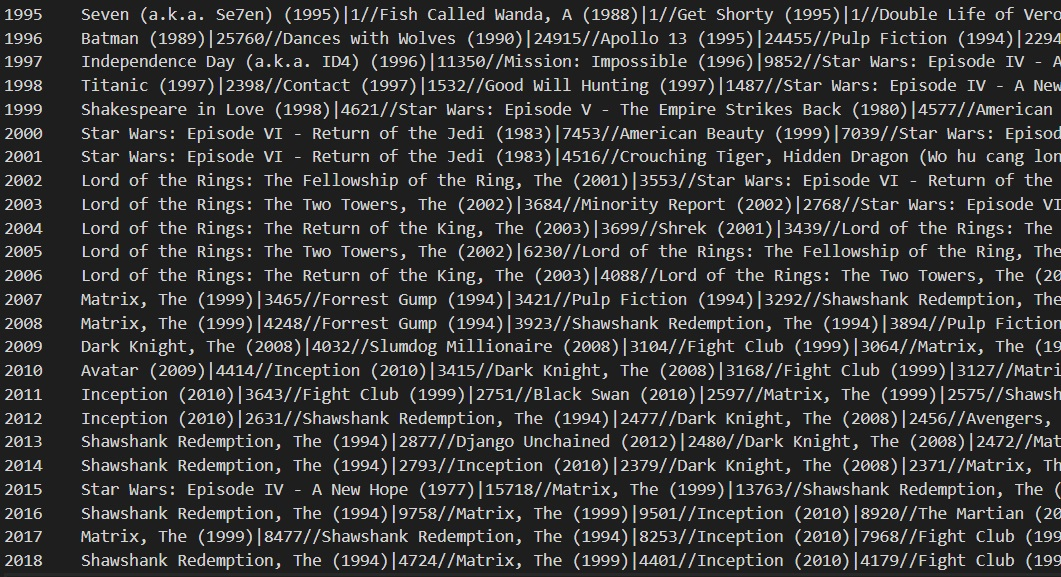
\includegraphics[scale=0.65]{images/Result2.jpg}
	\caption{Output ottenuto con il secondo job MapReduce}
	\label{Result2}
\end{figure}

\subsubsection{Spark implementation}

Per quanto riguarda l'implementazione del job realizzata in Spark, vale quanto detto relativamente alla query precedente. In questo caso risulta essere molto interessante la variabile broadcast contenente i record della tabella \textit{Movies}, che consente di eseguire l'operazione di join (con cui vengono aggiunti i titoli dei film al risultato) solo dopo aver selezionato gli N film con un numero di feeling più elevato e senza dover ripetere l'ordinamento (come in MapReduce).

Questo è possibile perché, con una variabile broadcast, la join si traduce in un'operazione \textit{mapValues} che va a modificare la lista di film associata ad ogni anno. Invece, se avessimo utilizzato un classico RDD contenente la tabella \textit{Movies}, per eseguire la join sarebbe stato necessario trasformare nuovamente l'RDD ottenuto dopo la selezione dei film, usando un record per ogni film (``appiattendo'' la lista associata ad ogni anno) e mettendo in chiave movieId.

Sia l'RDD contenente le valutazioni che quello contenente i tag sono stati esplicitamente partizionati attraverso un \textit{HashPartitioner}, in modo da evitare lo shuffling dei dati nelle due operazioni di \textit{reduceByKey} che seguono. Come si vede infatti dal DAG, grazie a questo partizionamento le due \textit{reduceByKey} sono eseguite nello stesso stage (\textit{mapValues} e \textit{union} sono operazioni eseguite localmente e che non prevedono un nuovo partizionamento dei dati).
 
La configurazione usata è la stessa del primo job implementato in Spark (2 executor, 3 core per executor e 2 gb di RAM) e il tempo di esecuzione totale, che comprende anche la prima query, è di 1 minuto e 54 secondi (\url{http://isi-vclust0.csr.unibo.it:18089/history/application_1583679666662_4566/jobs/}). Anche in questo caso il risultato ottenuto corrisponde a quello di MapReduce, con la differenza che in Spark ad ogni anno è associata una lista di tuple contenenti il titolo del film e il numero di feeling. Il file di testo prodotto in output è disponibile nella cartella \texttt{hdfs:/user/mmascellaro/outputSpark/query2}.

\begin{figure}[th]
	\centering
	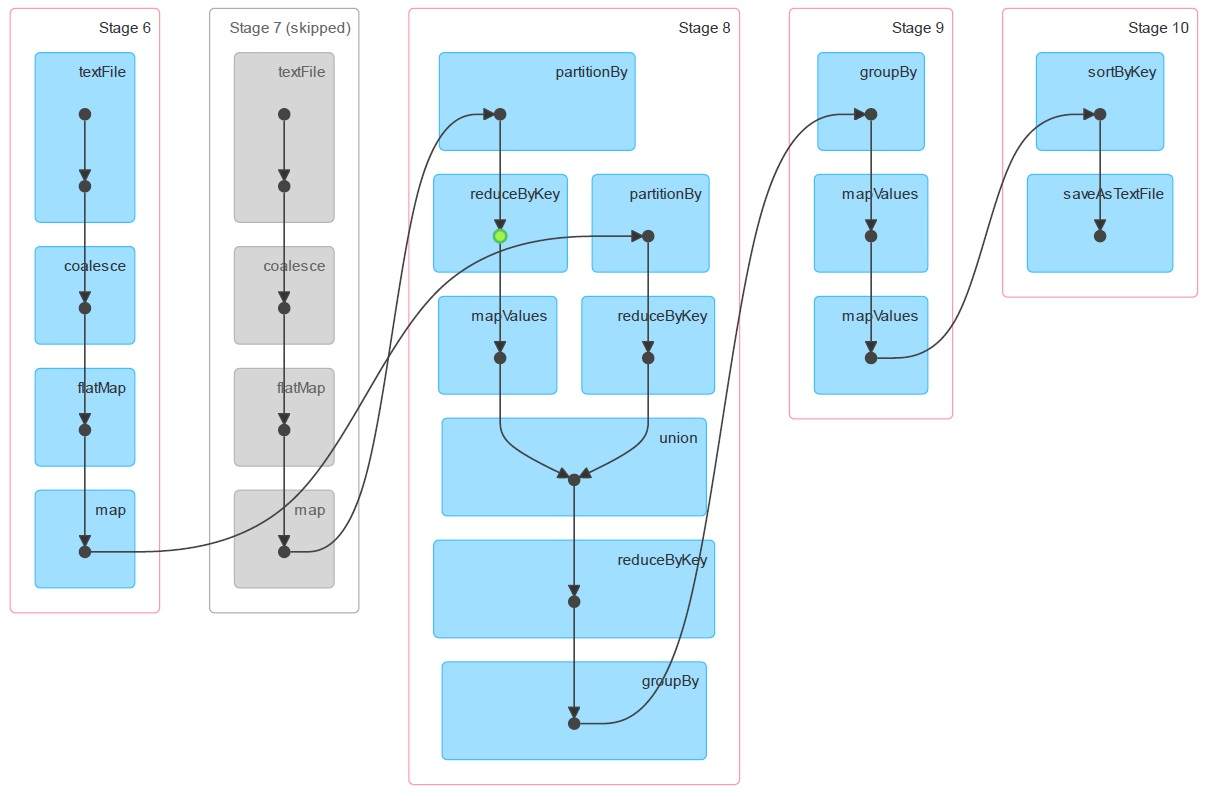
\includegraphics[scale=0.55]{images/DagSpark2.jpg}
	\caption{DAG relativo al secondo job Spark}
\end{figure}

\subsubsection{Spark SQL implementation}

Anche questo secondo job è stato implementato in Spark SQL, seguendo quanto già visto per il primo job e utilizzando le stesse configurazioni. Il tempo di esecuzione complessivo delle due query è stato di 2 minuti e 6 secondi (\url{http://isi-vclust0.csr.unibo.it:18089/history/application_1583679666662_4567/jobs/}) e l'output, memorizzato all'interno di un file \textit{json}, è disponibile all'interno della cartella \texttt{hdfs:/user/mmascellaro/outputSparkSQL/query2}.

\section{Performance considerations}

Per quanto riguarda le implementazioni MapReduce dei due job, il numero di reducer dei vari stage è stato scelto in seguito ad una serie di prove sperimentali riportate nella figura \ref{PerformanceMapReduce1}. In ognuna di queste prove i vari stage sono stati eseguiti con un numero di reducer pari a quello presente nella colonna della tabella, ad eccezione degli stage \textit{SortGenres} e \textit{SortMovies}. Questi ultimi, per la natura dell'interrogazione, sono stati eseguiti sempre con un unico reducer.

I tempi presenti nella tabella non corrispondono esattamente a quelli della versione finale (allegati alla descrizione dei job), poiché registrati in giornate diverse. Tuttavia, in ogni prova sono state utilizzate le ottimizzazioni applicate per MapReduce: i combiner e la vista pre-aggregata creata nello stage \#1.

È stata scelta una configurazione che prevede 4 reducer per il primo stage e 2 per tutti i rimanenti poiché, per il maggior volume di dati che devono essere trattati, il primo è l'unico in cui il vantaggio dato da un maggior numero di risorse compensa l'overhead dovuto alla distribuzione dei dati.

\begin{figure}[th]
	\centering
	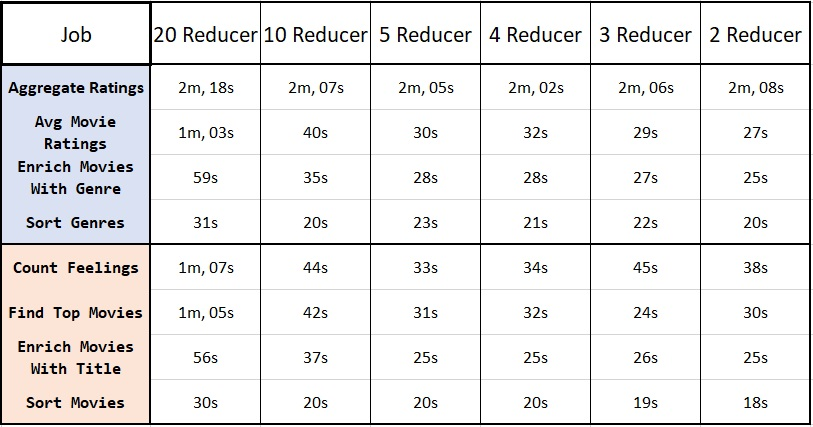
\includegraphics[scale=0.78]{images/PerformanceMapReduce1.jpg}
	\caption{Prove sperimentali eseguite con vari numeri di reducer}
	\label{PerformanceMapReduce1}
\end{figure}

Una volta scelta la configurazione (il numero di reducer per ogni stage), sono stati registrati i tempi relativi alla versione finale ed è stato valutato il vantaggio portato dalle ottimizzazioni. Come è possibile vedere dalla tabella presentata di seguito (\ref{PerformanceMapReduce2}), i combiner migliorano le prestazioni in ognuno degli stage in cui sono utilizzati e il miglioramento è più evidente quando il volume di dati trattato è maggiore. Provando invece ad eliminare lo stage \#1 e facendo in modo che i successivi leggessero soltanto dai file \textit{csv}, vi è stato un vantaggio di circa 35 secondi nella prima query ma un peggioramento maggiore di un minuto nella seconda. Questo evidenzia la bontà della creazione della vista pre-aggregata.

\begin{figure}[th]
	\centering
	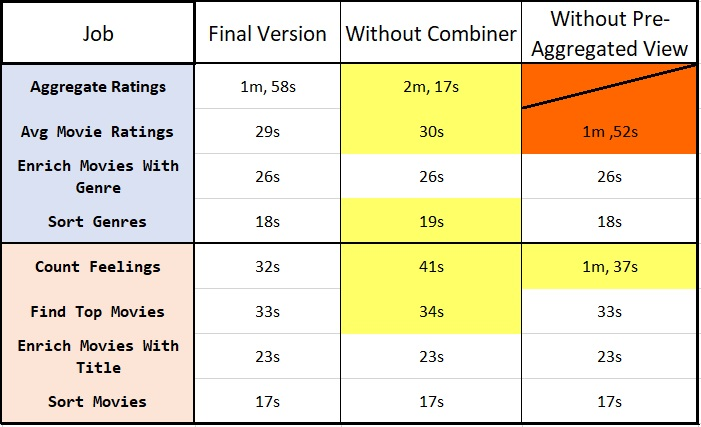
\includegraphics[scale=0.66]{images/PerformanceMapReduce2.jpg}
	\caption{Prestazioni ottenute con l'implementazione MapReduce}
	\label{PerformanceMapReduce2}
\end{figure}

Invece, in merito all'implementazione Spark, una volta realizzata la versione finale sono stati valutati i tempi assegnando ad ogni executor un numero di core compreso tra 1 e 4 (ogni nodo ha a disposizione 4 core). Si è notato un miglioramento aumentando il numero di core, e si è scelto di assegnare 3 core ad ogni executor in modo da lasciarne uno libero per l'esecuzione dei demoni.

Sia nei job Spark sia in quelli Spark SQL, l'uso della \textit{cache} ha portato vantaggi tangibili per quanto riguarda le performance. Inoltre, in Spark SQL un altro beneficio è stato ottenuto grazie alla modifica del numero di partizioni usate nella fase di shuffling. I tempi misurati sono riportati nella tabella \ref{PerformanceSpark}.

\begin{figure}[th]
	\centering
	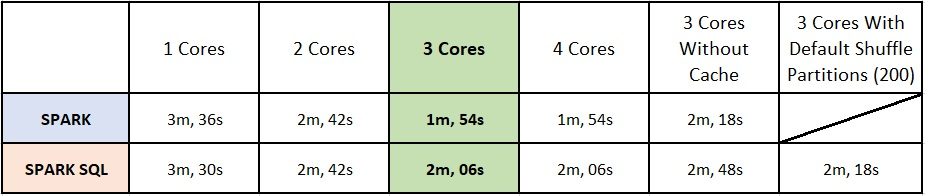
\includegraphics[scale=0.68]{images/PerformanceSpark.jpg}
	\caption{Prestazioni ottenute con Spark e Spark SQL}
	\label{PerformanceSpark}
\end{figure}

\end{document}
